\chapter{Introduction}
Autonomous netwoking is an advanced course built on existing knowledge. You should already have taken a standard computer networks course and be comfortable with the TCP/IP protocol stack, basic MAC layer mechanisms and routing protocols. Reasonable familiarity with probability and probabilistic thinking is also required, since many techniques we will discuss use stochastic models.

The course explores a variety of wireless, networked communication systems. We will study:
\begin{itemize}
    \item sensor networks;
    \item Internet of Things;
    \item backscattering networks such as RFID;
    \item unmanned networks (dronets).
\end{itemize}
A portion of the course focuses on reinforcement learning, because this is currently one of the most practical and compelling ways to design autonomous policies for networking tasks. We will first learn how to formalize reinforcement learning problems in a networking context. Then we will study specific techniques that apply broadly to networking: from bandit algorithms for simple decision problems to tabular and function-approximation variants of Q-learning for stateful environments.

\section{Why autonomous?}
Autonomy in networks carries multiple connotations. 
\begin{itemize}
    \item \textit{Self-Governance:} the system makes independent decisions based on predefined rules and real-time data rather than waiting for human intervention.
    \item \textit{Self-Sufficiency:} an autonomous network should be able to operate as an independent organism, managing its own resources and orchestrating tasks across nodes.
    \item \textit{Embedded intelligence:} autonomous systems integrate advanced algorithms, including machine learning, so they can interpret diverse environmental inputs, learn from past experiences and adapt their behavior as conditions change.
    \item \textit{Proactive Response:} an autonomous network continuously monitors its environment, anticipates disruptions and takes action to preserve or restore performance and reliability.
\end{itemize}

Consider a smart home with a lot of connected devices sharing a common wireless channel. Normally, the network carries routine traffic: temperature sensors, smart appliances and background media streaming. Imagine that someone starts a video stream that occupies most of the available bandwidth. Now imagine the smoke detector in the kitchen senses smoke. Devices monitoring the kitchen must be able to send their emergency data with minimal delay. An autonomous network should detect that this traffic is critical and change scheduling, prioritization or access policies so that kitchen sensors obtain channel access quickly and reliably. This is the kind of reactive and proactive behavior autonomous networking aims to provide.

\section{Which technologies?}
Most of our focus will be on wireless technologies that commonly require autonomy to satisfy strict constraints on latency, energy and reliability. These include:
\begin{itemize}
    \item \textit{Backscattering networks used in RFID systems:} Radio Frequency Identification, or RFID, is one of the simplest examples of a backscattering communication system. In RFID, very low-power tags communicate by reflecting a carrier transmitted by a reader (see Figure \ref{fig:rfid}).

    \begin{figure}[ht]
        \centering
        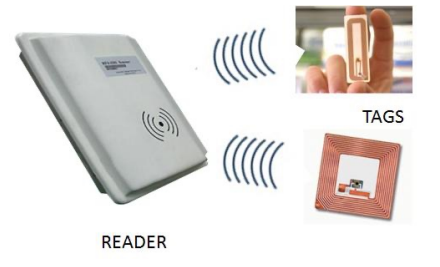
\includegraphics[width=0.4\linewidth]{images/rfid.png}
        \caption{Radio Frequency Identification - RFID.}
        \label{fig:rfid}
    \end{figure}
    \item \textit{Sensor and IoT:} Wireless sensor networks consist of a monitored area where spatially distributed sensors collect environmental data and forward it — often through multiple hops — to a central sink. The sink then relays information to servers or the Internet (see Figure \ref{fig:sensor-networks}).

    \begin{figure}[ht]
        \centering
        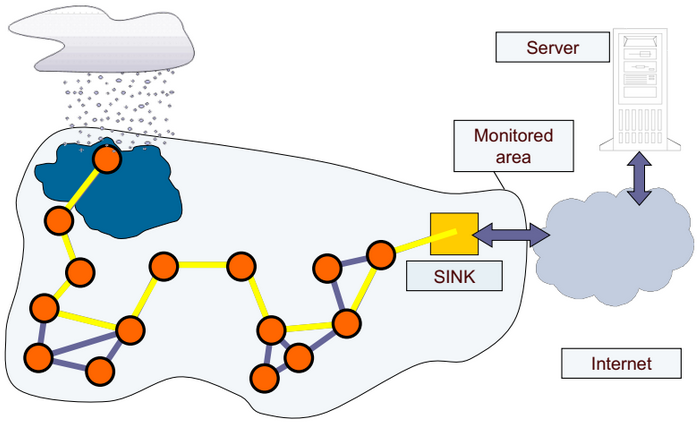
\includegraphics[width=0.6\linewidth]{images/sensor-network.png}
        \caption{Sensor networks.}
        \label{fig:sensor-networks}
    \end{figure}

    When we speak about IoT networks we are referring to heterogeneous collections of smart devices, sensors, RFID tags, Wi-Fi-enabled gadgets and gateways that form intelligent environments. Smart buildings and smart homes are canonical examples (see Figure \ref{fig:smart-city}). 
    
    \begin{figure}[ht]
        \centering
        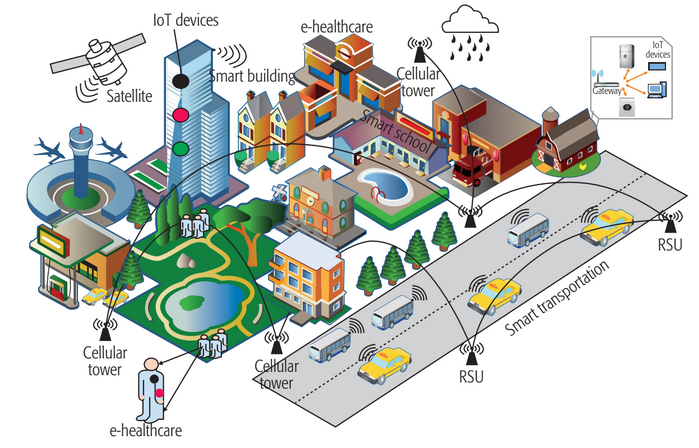
\includegraphics[width=0.7\linewidth]{images/smart-cities.png}
        \caption{Smart city.}
        \label{fig:smart-city}
    \end{figure}
    \item \textit{Unmanned networks (dronet):} Drones are used for many applications: to capture aerial images, to inspect structures, to experiment with parcel delivery and to collect data in places that would be hard to reach otherwise. Many of those applications still rely on a human pilot: someone at a remote control or a command center who makes most of the decisions. Yet there is a complementary vision in which drones operate as fully unmanned systems — squads of aerial vehicles that fly without a person physically present or constantly steering them.
\end{itemize}

\section{Autonomous means intelligent}
A common question is: how do we make a squad of drones or an IoT network autonomous? A short answer is: by giving the system learning and decision-making capabilities. One of the most natural frameworks to introduce that kind of intelligence is reinforcement learning.

\textit{Reinforcement learning}, or RL, addresses a simple but deep question: how can an intelligent agent learn to make a good sequence of decisions? That single sentence hides a lot. 
\begin{itemize}
    \item First, we are not concerned with one-off choices; instead, the agent must consider sequences where current actions influence the future. 
    \item Second, by saying a good sequence of decisions we implicitly mean there is some measure of utility or reward the agent seeks to maximize. 
    \item Third, the agent typically starts without a model of how its actions will affect the world; it has to learn that relationship by interacting with its environment.
\end{itemize}
Put differently, in RL the agent performs actions, observes consequences and receives feedback in the form of rewards. Over time, the agent should learn which actions tend to produce better long-term returns.

There are a few central themes you will hear repeatedly in RL: optimization, delayed consequences, exploration and generalization. Each of these themes maps directly to networking problems.
\begin{itemize}
    \item RL is an optimization problem: we want to find a policy — a way of making decisions — that yields the best outcome possible. In networks that objective could be throughput, latency, energy efficiency, fairness or some combination of metrics.
    \item A complicating factor is the temporal dimension: decisions taken now can ripple forward and affect rewards far in the future. Suppose an agent chooses to prioritize a low-latency flow now; that might make a future congestion episode worse. Planning and learning under such delayed consequences require us to identify correctly which actions were responsible for later successes or failures.
    \item Exploration is another practical challenge: agents learn about the world by trying things. In many real systems the learning data is censored — you only observe the outcome of decisions you actually took; you don't know what would have happened had you taken alternatives.
    \item Generalization is what allows an agent to cope with states it has never explicitly seen. A policy is, formally, a mapping from past experience to actions, so the agent must extract structure from past experience in order to act sensibly in new situations.
\end{itemize}
Equally important is robustness and risk sensitivity. Robustness refers to an agent’s ability to perform well under different, possibly unseen, conditions. Risk sensitivity captures how an agent handles uncertainty — whether it prefers conservative policies or aggressive policies.

By the end of the course you will be able to take a networking problem, such as a MAC or routing challenge, and decide whether it is appropriate to formulate it as an RL problem. If the answer is yes, you will be able to define the problem formally: specify the state space, action space, environment dynamics and reward model. You should also be able to select an algorithm from those we study and justify why that algorithm fits the problem constraints and objectives.